\documentclass[xcolor={dvipsnames}]{beamer}
\usetheme{Madrid}
\beamertemplatenavigationsymbolsempty


%%%% packages.tex by Stefano Gogioso 
%%%% Version 7 Dec 2016

\usepackage[toc,page]{appendix}
%% MATHS %%
\usepackage{mathtools} % Loads and extends amsmath
\usepackage{amssymb} % Extra mathematical symbols (loads amsfonts)
\usepackage{amsthm} % Theorem environments
\usepackage{stmaryrd} % Some maths symbols for logic and computer science
%\usepackage{cjhebrew} % Jewish symbols
%\usepackage[nodisplayskipstretch]{setspace} % Redefines spacing before/after equations

%% WRITING %%
\usepackage{relsize} % Additional relative sizes for fonts
\usepackage{microtype} % Improves appearance of writing
%\usepackage{fullpage} % Reduces lateral page margins for vanilla classes
\usepackage{multicol} % Multi-column environments
\usepackage{csquotes} % Environments for quotes
\usepackage{xspace}
%% CITATIONS %%
\usepackage{hyperref} % Hyperlink citations, comment out for arxiv submission 
\usepackage[nocompress]{cite} % Comment out if using natbib or apacite
\usepackage[hyperpageref]{backref} 
\renewcommand*{\backref}[1]{}
\renewcommand*{\backrefalt}[4]{%
	\ifcase #1 (Not cited.)%
	\or        (Cited on page~#2.)%
	\else      (Cited on pages~#2.)%
	\fi}
% QPL wants Bibtex!
% \usepackage[
% backend=biber,
% natbib=true,
% language=auto,
% style=numeric-comp,
% sorting=nyt,
% maxbibnames=10,
% firstinits=true,
% url=true, 
% doi=false,
% isbn=false,
% eprint=false
% ]{biblatex}

%\usepackage[sort&compress]{natbib} % Comment out if using cite or apacite
%\usepackage[round,authoryear,sort&compress]{natbib} % Comment out if using cite or apacite
%\usepackage{apacite} % Comment out if using natbib or cite

%% GRAPHICS %%
\usepackage{graphicx} % Import of graphics
\usepackage{subcaption} % Captioning and referencing sub-figures
\usepackage{wrapfig} % Figures wrapped in text
\usepackage[usenames,dvipsnames]{xcolor} % Introduces colour names
\usepackage{tikz} % TikZ
\usetikzlibrary{
	math,
	decorations.markings,
	positioning,
  arrows,
  intersections,
%	arrows.meta,
  shapes,
  shapes.misc,
	automata,
	petri,
	decorations,
	backgrounds,
	calc,
	fit,
	quotes
  }

  \usepackage{circuitikz}
%%%% macros.tex by Stefano Gogioso
%%%% Version 12 Apr 2017 


%% Theorem environments - Comment out for certain journal submissions and for beamer 
	%% Counters and miscellaneous
  \newcounter{theoremUnified} % Unified coutner for all theorem environments
  \def\thetheoremUnified{\arabic{section}} % Needed to have counters going with sections
  \numberwithin{theoremUnified}{section} % Numbering within sections
  \numberwithin{theoremUnified}{section} % Equations are also numbered within sections

% Theorem Styles
%
  \newtheoremstyle{plainStyle} % Plain theorem style
  {2mm} % Space above
  {2mm} % Space below
  {} % Body font
  {} % Indent amount
  {\bfseries} % Theorem head font
  {.} % Punctuation after theorem head
  {.5em} % Space after theorem head
  {} % Theorem head spec (can be left empty, meaning `normal')

  \newtheoremstyle{italicStyle} % Italic theorem style
  {2mm} % Space above
  {2mm} % Space below
  {\itshape} % Body font
  {} % Indent amount
  {\bfseries} % Theorem head font
  {.} % Punctuation after theorem head
  {.5em} % Space after theorem head
  {} % Theorem head spec (can be left empty, meaning `normal')

% Ubiquitous set names
\newcommand{\Naturals}{\mathbb{N}} % Set of natural numbers
\newcommand{\Integers}{\mathbb{Z}} % Set of interer numbers
\newcommand{\Bool}{\mathbb{B}} % Set of interer numbers

% Background for tikz images
\def\backgrnd{black!10}	% Background for Tikz pictures

% Basic Definitions
%
\newcommand{\Obj}[1]{\operatorname{Obj} \, #1} % Set of objects of category #1
\newcommand{\Mor}[1]{\operatorname{Mor} \, #1} % Set of objects of category #1
\newcommand{\GObj}[1]{\operatorname{GenObj} \, #1} % Set of objects of category #1
\newcommand{\GMor}[1]{\operatorname{GenMor} \, #1} % Set of objects of category #1

\newcommand{\Snark}[1]{\operatorname{Sn}(#1)} % Set of objects of category #1

\newcommand{\Homtotal}[1]{\operatorname{Hom}_{\,#1}} % Set of morphisms of category #1
\newcommand{\Hom}[3]{\operatorname{Hom}_{\,#1}\left[#2,#3\right]} % Set of morphisms of category #1 from object #2 to object #3
\newcommand{\Source}[2]{\operatorname{s}_{#1}(#2)} % Domain of function/morphism #1
\newcommand{\Target}[2]{\operatorname{t}_{#1}(#2)} % Domain of function/morphism #1
\newcommand{\Id}[1]{id_{#1}} % Identity morphism of object #1

% Generic names for categories
%
\newcommand{\CategoryA}{\mathcal{A}}
\newcommand{\CategoryB}{\mathcal{B}}
\newcommand{\CategoryC}{\mathcal{C}}
\newcommand{\CategoryD}{\mathcal{D}}
\newcommand{\CategoryE}{\mathcal{E}}

\newcommand{\Free}[1]{\mathfrak{F}(#1)}
\newcommand{\UnFree}[1]{\mathfrak{U}(#1)}

% Monoidal Categories
%
\newcommand{\Tensor}{\otimes} % Monoidal tensor
\newcommand{\TensorUnit}{I} % Monoidal tensor unit

% Logic
%
\newcommand{\Suchthat}[2]{\left\{#1 \: \middle\vert \: #2\right\}} % Set of elements #1 such that condition #2 holds 

% Category Names
\newcommand{\Bfun}{\Bool_\textbf{fun}} % Category of boolean functions
\newcommand{\Bcirc}{\Bool_\textbf{circ}} % Category of boolean circuits
\newcommand{\Bkp}{\Bool_\textbf{KP}} % Category of KP boolean circuits
\newcommand{\Bzkp}[1]{\Bool^{#1}_{\textbf{ZKP}}} % Category of KP boolean circuits

\newcommand{\Bpath}[1]{\Bool^{#1}_{\textbf{path}}} % Category of path proofs
\newcommand{\Count}{\textbf{Count}} % Category of KP boolean circuits
\newcommand{\Bgraph}[1]{\Bool^{#1}_{\Graph}} % Category of proof for a whole automaton
\newcommand{\Bsnark}{\Bool_\textbf{SNARK}} % Category of snark boolean circuits
\newcommand{\BsnarkSize}[1]{\Bool^{#1}_{\textbf{path}}} % Category of full snark proofs of some computational size

\newcommand{\Graph}{\textbf{Graph}} % Category of graphs
\newcommand{\Cat}{\textbf{Cat}} % Category of graphs

\newcommand{\NAND}{\ensuremath{\texttt{NAND}}\xspace}
\newcommand{\AND}{\ensuremath{\texttt{AND}}\xspace}
\newcommand{\NOT}{\ensuremath{\texttt{NOT}}\xspace}
\newcommand{\OR}{\ensuremath{\texttt{OR}}\xspace}
\newcommand{\XOR}{\ensuremath{\texttt{XOR}}\xspace}
\newcommand{\COPY}{\ensuremath{\texttt{COPY}}\xspace}
\newcommand{\TRUE}{\ensuremath{\texttt{TRUE}}\xspace}
\newcommand{\FALSE}{\ensuremath{\texttt{FALSE}}\xspace}
\newcommand{\Zero}{\ensuremath{\textbf{0}}\xspace}


\newcommand{\NANDSym}{
  \scalebox{0.3}{
    \tikz[baseline=-10pt] \node[thick, american nand port] (char) {};
  }
}

\newcommand{\XORSymb}{
  \scalebox{0.3}{
    \tikz[baseline=-10pt] \node[thick, american xor port] (char) {};
  }
}

\newcommand{\ANDSym}{
  \scalebox{0.3}{
    \tikz[baseline=-10pt] \node[thick, american and port] (char) {};
  }
}

\newcommand{\ORSym}{
  \scalebox{0.3}{
    \tikz[baseline=-10pt] \node[thick, american or port] (char) {};
  }
}
\newcommand{\COPYSym}{
  \scalebox{0.3}{
    \tikz[baseline=-8pt]{
      \node[thick, draw, circle, radius=2pt] (copy) at (0,0) {};
      \node (in) at (-1,0) {};
      \node (out1) at (1,0.5) {};            
      \node (out2) at (1,-0.5) {};
      \draw[thick, -] (in.center) to (copy);
      \draw[thick, -, bend left] (copy) to (out1.center);
      \draw[thick, -, bend right] (copy) to (out2.center);
    } 
  }
}

\newcommand{\MATCHSym}{
  \scalebox{0.3}{
    \tikz[baseline=-8pt]{
      \node[thick, draw, fill=gray, circle, radius=2pt] (copy) at (0,0) {};
      \node (in) at (1,0) {};
      \node (out1) at (-1,0.5) {};            
      \node (out2) at (-1,-0.5) {};
      \draw[thick, -, dotted] (in.center) to (copy);
      \draw[thick, -, bend right] (copy) to (out1.center);
      \draw[thick, -, bend left] (copy) to (out2.center);
    } 
  }
}

\tikzstyle{place}=
[circle,thick,draw=blue!75,fill=blue!20,minimum size=6mm]
\tikzstyle{transition}=
[rectangle,thick,draw=black!75,fill=black!20,minimum size=4mm]


\linespread{1}

\title[arxiv.org/abs/1909.02893]{Mapping Finite State Machines to zk-SNARKs \\ Using Category Theory}
\subtitle{A talk for DEVCON V}
\author[Genovese, Knispel, Fitzgerald]{Fabrizio Genovese, Andre Knispel, Joshua Fitzgerald}
\institute[ ]{Statebox Team}
\date[Twitter: \texttt{@statebox}]{8 Oct 2019, Osaka JP \\ arxiv.org/abs/1909.02893\\ \vspace{0.8em}\includegraphics[height=2cm]{logo.png}}
%
%
%
\begin{document}
%
%
%
\setbeamercolor{background canvas}{bg=CarnationPink!50}	
\begin{frame}
	\titlepage
\end{frame}
%
%
\begin{frame}{What is a zk-SNARK??}
  %
  zk-SNARKs are a way to prove that some computation followed some
  rules, without revealing anything of the computation itself.\pause
  %
  %
  \begin{itemize}
    \item They are good for privacy!
      \pause
    \item They compress information by a lot;
      \pause
    \item Blockchain people seem to love them.
      \pause
  \end{itemize}
  %

  \bigskip
  Knowing what a zk-SNARK is is not important for this talk! \pause

  \bigskip
  What is important is to know that if you have a \textbf{boolean circuit},
  then you can turn it into a zk-SNARK.
\end{frame}
%
%
\begin{frame}{...Then what is a boolean circuit?}
 % 
  \pause
  Literally, a bunch of logical gates wired together. \pause
  %
  %
  \begin{equation*}
    \scalebox{0.5}{
    \tikz[baseline]{
      \node[american nand port] (nand) at (1.5,0) {};
      \node at ([xshift=5pt]nand.out) {$X$};
      \node at (0,0.3) {$X$} ;
      \node at (0,-0.3) {$X$} ;
    }}
    \qquad
    \scalebox{0.5}{
    \tikz[baseline]{
      \node[thick, draw, circle, radius=2pt] (copy) at (0,0) {};
      \node[label={[label distance=-10pt]180:$X$}] (in) at (-1,0) {};
      \node[label={[label distance=-10pt]0:$X$}]  (out1) at (1,0.5) {};            
      \node[label={[label distance=-10pt]0:$X$}]   (out2) at (1,-0.5) {};
      \draw[thick, -] (in) to (copy);
      \draw[thick, -, bend left] (copy) to (out1);
      \draw[thick, -, bend right] (copy) to (out2);
    }}
    \qquad
    \scalebox{0.5}{
    \tikz[baseline]{
      \node[american or port] (nand) at (1.5,0) {};
      \node at ([xshift=5pt]nand.out) {$X$};
      \node at (0,0.3) {$X$} ;
      \node at (0,-0.3) {$X$} ;
    }}
    \qquad
    \scalebox{0.5}{
    \tikz[baseline]{
      \node[thick, draw, circle, radius=2pt, inner sep = 2pt] (true) at (0,0) {\tiny{$\bot$}};
      \node[label={[label distance=-10pt]0:$X$}] (out) at (1,0) {};            
      \draw[thick, -] (copy) to (out);
    }}
  \end{equation*}\pause

  \begin{center}
    \resizebox{6cm}{2.5cm}{
    \begin{circuitikz}[baseline=70pt]
      \draw (-1,2.14)  node[american not port, scale = 0.3] (a1){};
      \draw (-1,3.14)  node[american not port, scale = 0.3] (a2){};
      \draw (-1,3.86)  node[american not port, scale = 0.3] (a3){};
      \draw (-1,4.86)  node[american not port, scale = 0.3] (a4){};
    
      \draw (0,0)  node[american and port, scale = 0.5] (b1){};
      \draw (0,1) node[american and port, scale = 0.5] (b2){};
      \draw (0,2)  node[american and port, scale = 0.5] (b3){};
      \draw (0,3) node[american and port, scale = 0.5] (b4){};
      \draw (0,4)  node[american and port, scale = 0.5] (b5){};
      \draw (0,5) node[american and port, scale = 0.5] (b6){};
    
      \draw (1,0.5)  node[american and port, scale = 0.5] (c1){};
      \draw (1,2.5)  node[american and port, scale = 0.5] (c2){};
      \draw (1,4.5)  node[american and port, scale = 0.5] (c3){};
    
      \draw (2,1.5)  node[american or port, scale = 0.5] (d1){};
    
      \draw (3,2.5)  node[american or port, scale = 0.5] (e1){};
    
      \draw[-] (d1.out) |- (e1.in 2);
      \draw[-] (c3.out) |- (e1.in 1);
    
      \draw[-] (c1.out) |- (d1.in 2);
      \draw[-] (c2.out) |- (d1.in 1);
    
      \draw[-] (b1.out) |- (c1.in 2);
      \draw[-] (b2.out) |- (c1.in 1);
      \draw[-] (b3.out) |- (c2.in 2);
      \draw[-] (b4.out) |- (c2.in 1);
      \draw[-] (b5.out) |- (c3.in 2);
      \draw[-] (b6.out) |- (c3.in 1);
    
      \draw[-] (a1.out) |- (b3.in 1);
      \draw[-] (a2.out) |- (b4.in 1);
      \draw[-] (a3.out) |- (b5.in 2);
      \draw[-] (a4.out) |- (b6.in 2);
    
      \draw[-*] let \p1=(b1.in 2) in (-3,6) to ([yshift=-2pt]-3,\y1);
      \draw[-] let \p1=(b1.in 2) in (-3,\y1) to (b1.in 2);
      \draw[-*] let \p1=(b1.in 1) in (-2.5,6) to ([yshift=-2pt]-2.5,\y1);
      \draw[-] let \p1=(b1.in 1) in (-2.5,\y1) to (b1.in 1);
      \draw[-*] let \p1=(b2.in 2) in (-2,6) to ([yshift=-2pt]-2,\y1);
      \draw[-] let \p1=(b2.in 2) in (-2,\y1) to (b2.in 2);
      \draw[-*] let \p1=(b2.in 1) in (-1.5,6) to ([yshift=-2pt]-1.5,\y1);
      \draw[-] let \p1=(b2.in 1) in (-1.5,\y1) to (b2.in 1);
      
      \draw[-*] let \p1=(a1.in) in (-2.5,6) to ([yshift=-2pt]-2.5,\y1);
      \draw[-] let \p1=(a1.in) in (-2.5,\y1) to (a1.in);
      \draw[-*] let \p1=(b3.in 2) in (-3,6) to ([yshift=-2pt]-3,\y1);
      \draw[-] let \p1=(b3.in 2) in (-3,\y1) to (b3.in 2);
      
      \draw[-*] let \p1=(a2.in) in (-1.5,6) to ([yshift=-2pt]-1.5,\y1);
      \draw[-] let \p1=(a2.in) in (-1.5,\y1) to (a2.in);
      \draw[-*] let \p1=(b4.in 2) in (-2,6) to ([yshift=-2pt]-2,\y1);
      \draw[-] let \p1=(b4.in 2) in (-2,\y1) to (b4.in 2);
      
      \draw[-*] let \p1=(a3.in) in (-3,6) to ([yshift=-2pt]-3,\y1);
      \draw[-] let \p1=(a3.in) in (-3,\y1) to (a3.in);
      \draw[-*] let \p1=(b5.in 1) in (-2.5,6) to ([yshift=-2pt]-2.5,\y1);
      \draw[-] let \p1=(b5.in 1) in (-2.5,\y1) to (b5.in 1);
      \draw[-*] let \p1=(a4.in) in (-2,6) to ([yshift=-2pt]-2,\y1);
      \draw[-] let \p1=(a4.in) in (-2,\y1) to (a4.in);
      \draw[-*] let \p1=(b6.in 1) in (-1.5,6) to ([yshift=-2pt]-1.5,\y1);
      \draw[-] let \p1=(b6.in 1) in (-1.5,\y1) to (b6.in 1);
    \end{circuitikz}}
  \end{center}
  %
\end{frame}
%
%
\begin{frame}{What is a Finite State Machine (FSM)?}
 % 
  \pause
  \begin{center}
    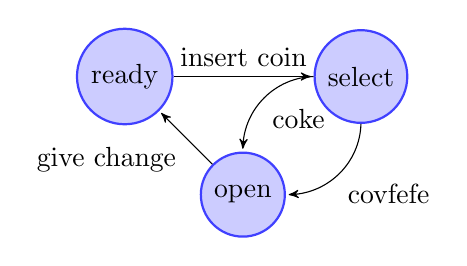
\begin{tikzpicture}[node distance=1.3cm,>=stealth',bend angle=45,auto]
      \node[place] (1) at (0,0) {ready};
      \node[place] (2) at (3,0) {select}
        edge [pre] node[swap] {insert coin} (1);
      \node[place] (3) at (1.5,-1.5) {open}
        edge [pre, bend left] node[swap] {coke} (2)
        edge [pre, bend right] node[swap] {covfefe} (2)
        edge [post] node {give change} (1);
    \end{tikzpicture}
  \end{center}
  %
  A FSM is some very old and cute thing in theoretical computer science.\pause

  \medskip
  For us, a FSM will just be a graph:
    \pause
  %
  %
  \begin{itemize}
    \item Vertexes of the graphs represent states of the FSM;
      \pause
    \item An arc between two vertexes represents an operation that mutates the state of the FSM;
      \pause
    \item A computation that follows the rules of the FSM is just a path on the graph.
      \pause
  \end{itemize}
  %
  If we can map graph paths to boolean circuits, then we can get a zk-SNARK verifying
  that a given computation followed the FSM rules!
  %
\end{frame}
%
%
\begin{frame}{Yeah but WTF is category theory anyway?}
  %
  \pause
  Category theory is a very complicated way to do simple things.
    \pause

  \bigskip
  The reason why it's cool is that it scales better than traditional maths, so 
  super-complicated things are actually easier when done categorically.
    \pause
  
  \bigskip
  Also, it's super related to type theory, so functional programming people love it, and functional programming is cool.
    \pause
  
  \bigskip
  Category theory allows to relate different mathematical structures compositionally:
  That is, in a way that respects the structure of the things we are relating.
\end{frame}
%
%
\begin{frame}{This means that...}
  \pause
  %
  If we build a categorical correspondence between graphs and boolean circuits,
  then we can be sure that if we morph the graph the circuit will morph accordingly.\pause

  \bigskip
  Moreover, once categorified concepts are automatically related to all mathematics:
  If you have a categorical way to map what you care about to graphs, then you automatically
  have a way to map that thing to boolean circuits (and hence to get a zk-SNARK for it!)
\end{frame}
%
%
\begin{frame}{The category of paths for a graph}
  Each graph $G$ can be used to build a category $\Free{G}$, which represents all the possible paths in the graph:
  %
  %
  \begin{center}
    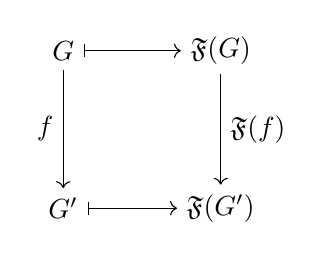
\begin{tikzpicture}
      \node (1) at (0,2) {$G$};
      \node (2) at (2,2) {$\Free{G}$};
      \node (3) at (0,0) {$G'$};
      \node (4) at (2,0) {$\Free{G'}$};
      \draw[->] (1) -- node[midway, left] {$f$} (3);
      \draw[->] (2) -- node[midway, right] {$\Free{f}$} (4);
      \draw[|->] (1) -- node[midway] {} (2);
      \draw[|->] (3) -- node[midway] {} (4);
    \end{tikzpicture}  
  \end{center}
  %
\end{frame}
%
%
\begin{frame}{Circuits from graphs}
  We can use the adjacency matrix of a graph $G$ to build a circuit:
  %
  %
  \begin{equation*}
    \scalebox{0.75}{
    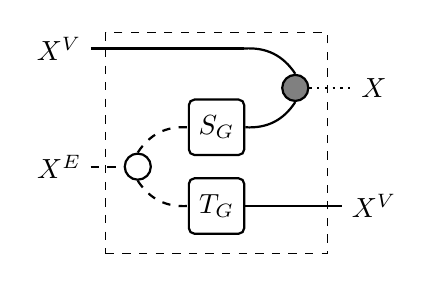
\begin{tikzpicture}
      \node[draw, circle, radius=5pt, thick] (copy) at (-1,0.5) {};
      \node[draw, minimum height=20, minimum width=20, rounded corners=2, thick] (S) at (0,1) {$S_G$};
      \node[draw, minimum height=20, minimum width=20, rounded corners=2, thick] (T) at (0,0) {$T_G$};
      \node[draw, fill=gray, circle, radius=5pt, thick] (mat) at (1,1.5) {};
  
      \node[draw, dashed, minimum height=80, minimum width=80] (contour) at (0,0.8) {};
  
      \node (Xv) at (-2,2) {$X^V$};
      \node (Xe) at (-2,0.5) {$X^E$};
      \node (X) at (2,1.5) {$X$};
      \node (Xv2) at (2,0) {$X^V$};
  
      \draw[-, thick] (Xv) to (10pt,2);
      \draw[bend left, thick] (10pt,2) to (mat.north);
      \draw[bend right, thick] (S.east) to (mat.south);
  
      \draw[dashed, -, thick] (Xe) to (copy.west);
  
      \draw[dashed, bend left, thick] (copy.north) to (S.west);
      \draw[dashed, bend right, thick] (copy.south) to (T.west);
  
      \draw[-, dotted, thick] (mat.east) -- (X);
      \draw[-, thick] (T.east) -- (Xv2.west);
    \end{tikzpicture}}
  \end{equation*}
  %
  \pause

  The left wires receive the enumeration of a vertex (top), and of an edge (bottom) respectively.\pause

  \medskip
  The wire up right returns 1 if the vertex is the source of the edge, 0 otherwise.  The bottom right wire returns the target vertex of the edge.
  \pause

  \medskip
  We can clearly compose these circuits by piping them one into the other.
  For each category of paths $\Free{G}$, we are are able to get a functor
  -- a structure preserving map -- to the category of boolean circuits.
\end{frame}
\begin{frame}{Generalizing over graphs}
  We can abstract over the adjacency matrix obtaining the following circuit:

  \begin{center}
    \scalebox{0.75}{
    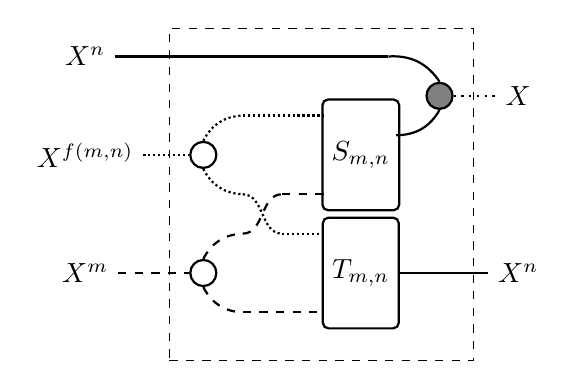
\begin{tikzpicture}
      \node[draw, circle, radius=5pt, thick] (copy2) at (-2,1.75) {};
      \node[draw, circle, radius=5pt, thick] (copy) at (-2,0.25) {};

      \node[draw, minimum height=40, minimum width=20, rounded corners=2, thick] (S) at (0,1.75) {$S_{m,n}$};
      \node[draw, minimum height=40, minimum width=20, rounded corners=2, thick] (T) at (0,0.25) {$T_{m,n}$};
      \node[draw, fill=gray, circle, radius=5pt, thick] (mat) at (1,2.5) {};

      \node[draw, dashed, minimum height=120, minimum width=110] (contour) at (-0.5,1.25) {};

      \node (Xv) at (-3.5,3) {$X^n$};
      \node (Xf) at (-3.5,1.75) {$X^{f(m,n)}$};
      \node (Xe) at (-3.5,0.25) {$X^m$};

      \node (X) at (2,2.5) {$X$};
      \node (Xv2) at (2,0.25) {$X^n$};

      \draw[-, thick] (Xv) to (10pt,3);
      \draw[-, densely dotted, thick] (Xf) to (copy2.west);
      \draw[-, dashed, thick] (Xe) to (copy.west);

      \draw[densely dotted, bend left, thick] (copy2.north) to (-1.5,2.25);
      \draw[densely dotted, bend right, thick] (copy2.south) to (-1.5, 1.25);
      \draw[dashed, bend left, thick] (copy.north) to (-1.5,0.75);
      \draw[dashed, bend right, thick] (copy.south) to (-1.5, -0.25);

      \draw[-, densely dotted, thick] (-1.5, 2.25) to (-0.47, 2.25);
      \draw[dashed, thick, out=0, in=180] (-1.5,0.75) to (-1, 1.25);
      \draw[densely dotted, thick, out=0, in=180] (-1.5,1.25) to (-1,0.75);
      \draw[-, dashed, thick] (-1.5, -0.25) to (-0.47,-0.25);

      \draw[-, dashed, thick] (-1, 1.25) to (-0.47, 1.25);
      \draw[-, densely dotted, thick] (-1, 0.75) to (-0.47,0.75);

      \draw[bend left, thick] (10pt,3) to (mat.north);
      \draw[bend right, thick] (0.45, 2) to (mat.south);

      \draw[dashed, -, thick] (Xe) to (copy.west);



      \draw[-, dotted, thick] (mat.east) -- (X);
      \draw[-, thick] (T.east) -- (Xv2.west);
    \end{tikzpicture}}
  \end{center}
    \pause
  The second wire on the left accepts a specification of an adjacency matrix of $m \times n$ bits.
  After having specified this, the circuit behaves like the one in the previous slide. 
    \pause
    
  \bigskip
    Again the circuits are composable and we obtain a functor from the category of graphs to the category 
    of boolean circuits.
\end{frame}
\begin{frame}{The power of category theory}
  Everything we built is compositional!!
  %
  %
  \begin{center}
    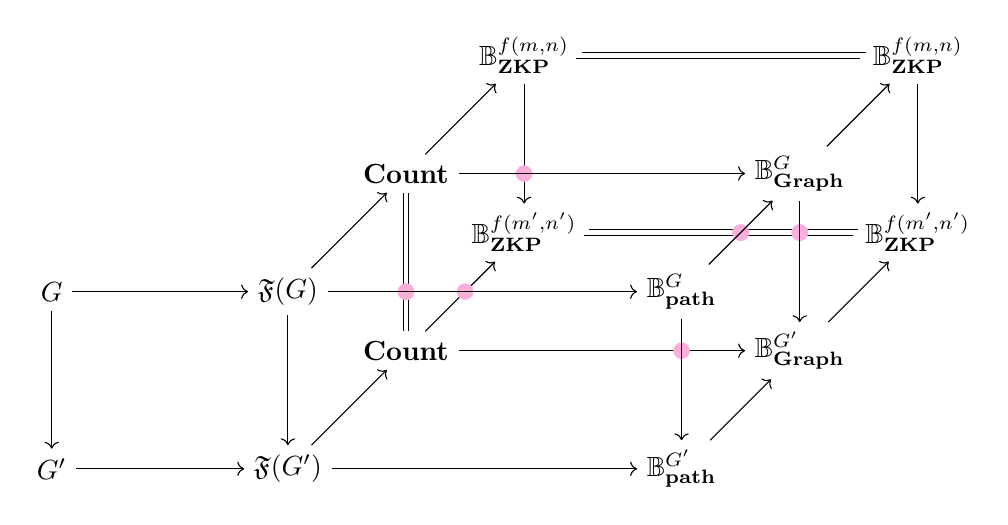
\begin{tikzpicture}
      \pgfdeclarelayer{fg}
      \pgfdeclarelayer{crossing}
      \pgfdeclarelayer{bg}
      \pgfsetlayers{main,bg,crossing,fg}
      %
      \node (G') at (0,0) {$G'$};
      \node(G) at (0,2.25) {$G$};
      \node(FG') at (3,0) {$\Free{G'}$};
      \node(FG) at (3,2.25) {$\Free{G}$};
      \node(Bpath') at (8,0) {$\Bpath{G'}$};
      \node(Bpath) at (8,2.25) {$\Bpath{G}$};
      \node(Count') at (4.5,1.5) {$\Count$};
      \node(Count) at (4.5,3.75) {$\Count$};
      \node(Bzkp') at (6,3) {$\Bzkp{f(m',n')}$};
      \node(Bzkp) at (6,5.25) {$\Bzkp{f(m,n)}$};
      \node(Bgraph') at (9.5,1.5) {$\Bgraph{G'}$};
      \node(Bgraph) at (9.5,3.75) {$\Bgraph{G}$};
      \node(Bzkp1') at (11,3) {$\Bzkp{f(m',n')}$};
      \node(Bzkp1) at (11,5.25) {$\Bzkp{f(m,n)}$};
      % Top
        \draw[->] (G) -- (FG);
        \draw[->] (FG) -- (Count);
        \draw[->] (Count) -- (Bzkp);
        \draw[transform canvas={yshift=-1pt, xshift=-1pt}, =] (Bzkp) -- (Bzkp1);
        \draw[transform canvas={yshift=1pt, xshift=1pt}, =] (Bzkp) -- (Bzkp1);
        \draw[->]  (Bgraph) -- (Bzkp1) ;
      % Bottom
        \draw[->] (G') -- (FG');
        \draw[->] (FG') -- (Bpath');
        \draw[->] (FG') -- (Count');
        \draw[->] (Bgraph') --  (Bzkp1');
        \draw[->] (Bpath') -- (Bgraph');
      % Vertical
        \draw[->] (G) -- (G');
        \draw[->] (FG) -- (FG');
        \draw[->] (Bzkp1) -- (Bzkp1');
      %FG
      \begin{pgfonlayer}{fg}
        \draw[->, name path global/.expanded=fgbpath] (FG) -- (Bpath);
        \draw[->, name path global/.expanded=countbgraph] (Count) -- (Bgraph);
        \draw[->, name path global/.expanded=bgraphbpath] (Bpath) -- (Bgraph);
        \draw[->, name path global/.expanded = bgraphbgraph'] (Bgraph) -- (Bgraph');
        \draw[->, name path global/.expanded=bpathbpath'] (Bpath) -- (Bpath');
      \end{pgfonlayer}
    %BG
      \begin{pgfonlayer}{bg}
        \draw[-> , name path global/.expanded=countbzkp'] (Count') -- (Bzkp');
        \draw[->, name path global/.expanded=countbgraph'] (Count') -- (Bgraph');
        \draw[transform canvas={yshift=-1pt, xshift=-1pt}, =, name path global/.expanded=bzkpid1] (Bzkp') -- (Bzkp1');
        \draw[transform canvas={yshift=1pt, xshift=1pt}, =, name path global/.expanded=bzkpid2] (Bzkp') -- (Bzkp1');
        \draw[transform canvas={xshift=-1pt}, =, name path global/.expanded=countcount'1] (Count) -- (Count');
        \draw[transform canvas={xshift=1pt}, =, name path global/.expanded=countcount'2] (Count) -- (Count');
        \draw[->, name path=bzkpbzkp'] (Bzkp) -- (Bzkp');
      \end{pgfonlayer}
      % Intersections
      \begin{pgfonlayer}{crossing}
        \fill[CarnationPink!50, name intersections={of=bgraphbpath and bzkpid1, name=i}] (i-1) circle (3pt);
        \fill[CarnationPink!50, name intersections={of=bgraphbpath and bzkpid2, name=i}] (i-1) circle (3pt);
        \fill[CarnationPink!50, name intersections={of=bgraphbgraph' and bzkpid1, name=i}] (i-1) circle (3pt);
        \fill[CarnationPink!50, name intersections={of=bgraphbgraph' and bzkpid2, name=i}] (i-1) circle (3pt);
        \fill[CarnationPink!50, name intersections={of=fgbpath and countbzkp', name=i}] (i-1) circle (3pt);
        \fill[CarnationPink!50, name intersections={of=countbgraph' and bpathbpath', name=i}] (i-1) circle (3pt);
        \fill[CarnationPink!50, name intersections={of=bzkpbzkp' and countbgraph, name=i}] (i-1) circle (3pt);
        \fill[CarnationPink!50, name intersections={of=countcount'1 and fgbpath, name=i}] (i-1) circle (3pt);
        \fill[CarnationPink!50, name intersections={of=countcount'2 and fgbpath, name=i}] (i-1) circle (3pt);
      \end{pgfonlayer}
      %
      \end{tikzpicture}
  \end{center}
\end{frame}

\begin{frame}{Take home message:}
    \pause
  When you do things categorically there's a good chance that:
    \pause
  %
  %

  \bigskip
  \begin{itemize}
    \item They will be formally correct; 
      \pause
    \item You will be able to verify that your constructions satisfy some nice properties;  
      \pause
    \item They will be more easily implementable in a formally verified setting, since already well structured;
      \pause
    \item You will be able to link things together without making a mess.
      \pause
  \end{itemize}
  %

  \bigskip
  Category theory seems difficult in the beginning, but it's just a better method to do software engineering!
\end{frame}
{
	\usebackgroundtemplate{\includegraphics[width=\paperwidth]{End.jpg}}%
	\begin{frame}
	
	\end{frame}
}	


\end{document}

